% This is LLNCS.DEM the demonstration file of
% the LaTeX macro package from Springer-Verlag
% for Lecture Notes in Computer Science,
% version 2.4 for LaTeX2e as of 16. April 2010
%

\documentclass{llncs}
%
\usepackage{makeidx}  % allows for indexgeneration
\usepackage[pdftex]{graphicx}
% declare the path(s) where your graphic files are
\graphicspath{{./Images/}}
% and their extensions so you won't have to specify these with
% every instance of \includegraphics[scale=•]{•}
\DeclareGraphicsExtensions{.jpeg,.jpg,.png}

\usepackage{url}
\urldef{\mailsa}\path|jane.jovanovski@gmail.com, maja.siljanoska@gmail.com, carevski@gmail.com, dragan.sahpaski@gmail.com, pgorcevski@t-home.mk, metodi.micev@gmail.com, b.ilijoski@gmail.com, vlatko.gmk@gmail.com|
\usepackage[pdfpagelabels,hypertexnames=false,breaklinks=true,bookmarksopen=true,bookmarksopenlevel=2]{hyperref}

\begin{document}

\mainmatter

%
% paper title
% can use linebreaks \\ within to get better formatting as desired
\pagestyle{plain}
\thispagestyle{plain}
\pagenumbering{arabic}

\title{Formal Methods Technical Report}

% the name(s) of the author(s) follow(s) next
%
% NB: Chinese authors should write their first names(s) in front of
% their surnames. This ensures that the names appear correctly in
% the running heads and the author index.
%
%
% NB: a more complex sample for affiliations and the mapping to the
% corresponding authors can be found in the file "lnicst.dem",
% that is contained in the LNICST LaTeX support package.
%

% author names and affiliations

\author{
Jane Jovanovski \and Maja Siljanoska\and Vladimir Carevski 
\and \\ Dragan Sahpaski \and Petar Gjorcevski \and Metodi Micev 
\and \\ Bojan Ilijoski \and Vlado Georgiev  
}  %

% the affiliations are given next
\institute{Institute of Informatics,\\
Faculty of Natural Sciences and Mathematics,\\
University "Ss. Cyril and Methodius",\\
Skopje, Macedonia\\
\mailsa
}

\maketitle

\begin{abstract}
%\boldmath
The Calculus of Communicating Systems (CCS) is a young branch in process calculus introduced 
by Robin Milner. CCS's theory has promising results in the field of modeling and analysing 
of reactive systems. Despite CCS's success, there are only few computer tools that are available
for modeling and analysis of CCS's theory. This paper is a technical report of an effort to
build such a tool. The tool is able to parse CCS's expressions, it can build LTSs 
(Labelled Transition Systems) from expressions and it can calculate if two LTS are bisimular
by using naive method or by using Fernandez's method. The tool is simple, but it has the 
functionality needed to perform modeling, specification and verification of certain system.

\keywords{Reactive Systems, CCS, Formal Methods, Process Algebra}

\end{abstract} % Abstract
\section{Introduction}

(The tool is a Java executable jar library with very simple user interface...)

TODO: Rewrite the introduction to represent a longer summary of the report. 

\subsection{Related work} 

In the past two decades different tools for modeling, specification and verification of concurrent reactive systems 

The Edinburgh Concurrency Workbench (CWB) is a tool for analysis of cuncurrent systems. CWB allows for equivalence, preorder and model checking using a variety of different process semantics. It also allows defining of behaviours in an extended version of CCS and perform various analysis of these behaviours, such as checking various semantic equivalences for examples checking if two processes (agents in CWB) are strongly or weakly bisimilar \cite{CWB}. Although CWB covers much of the functionality of our tool and more, CWB has a command interpreter interface that is more difficult to work with, unlike our tool that has a Graphical User Interface (GUI), and is very intuitive. As far as we know the CWB does not have the functionality for exporting LTS graphs in Aldebaran format, that our tool has. We have used the CWB many times while testing our tool, for checking CCS validity and also testing algorithms for strong and weak bisimularity of LTS graphs. 

The micro Common Representation Language 2 (mCRL2), successor of �CRL, is a formal specification language that can be used to specify and analyse the behaviour of distrubuted systems and protocols. Its accompanying toolset contains extensive collection of tools to automatically translate any mCRL2 specification to a linear process, manipulate and simulate linear processes, generate the state space associated with a linear process, manipulate and visualize state spaces, generate a PBES from a formula and a linear process, generate a BES from PBES and manipulate and solve (P)BESs \cite{mCRL2}. All mCRL2 tools can be used from the command line, but mCRL2 has an enhanced Graphical User Interface (GUI) as well which makes it very user-friendly and easy and to use. However, to our knowledge, mCRL2 does not provide the possibility to define systems' behaviour in the CCS process language nor to specify systems' properties using HML logic, functionalities that are implemented in the very initial version of our tool. Also, even though mCRL2 supports minimization modulo strong and weak bisimulation equivalence, it does not output the computed bisimulation, feature that we have implemented in our tool.
 
\subsection{Outline} The contributions of this paper are organized as follows. In the next section we give introduction to some of the basic terminology used throughout the report. The third section is devoted to the implementation of the CCS process language and generation of Labelled Transition Systems as a semantic model of process expressions, and it also discusses some of the choices made during the implementation. Section four describes the process of reducing the size of the state space of an LTS as well as checking the equivalence between two LTSs with respect to behavioural relations such as strong bisimilarity and observational equivalence (weak bisimilarity). It includes implementation details of two algorithms for computing strong bisimulation equivalence, the naive algorithm and the advanced algorithm due to Fernandez, as well as description of the saturation technique together with a respective algorithm  for saturating an LTS with which the problem of computing weak bisimilarity is reduced to computing strong bisimilarity over the saturated systems. Section five explains how the implementation of Hennesy-Milner Logic (HML) works and gives implementation details for the $U_{w}$ and $U_{s}$ operators. Next we illustrate the application of the tool for modeling, specification and verification of some classical examples. These classical examples include the Alternating Bit Protocol and Peterson's mutual exclusion algorithm. Finally, we give some conclusions and some directions for future development of the tool. We also include four appendixes. The first appendix contains the experimental results we got with analysis of the running times of our implementations of the two algorithms for computing bisimulation equivalence. The second one shows the syntax diagram for the grammar that recognizes CCS expressions . And the last appendix includes some visual illustration of the tool's usage via screenshots of the graphical application.
 % Chapter1
\section{CCS parsing and labeled transition system generation}
\label{sec:parsing}

Given a set of action names, the set of CCS processes is defined by the following BNF grammar:

\begin{equation}\label{eq:ccs_bnf}
P ::= \emptyset \hspace{1 mm} | \hspace{1 mm} a.P_{1} \hspace{1 mm} | \hspace{1 mm} A \hspace{1 mm} | \hspace{1 mm}P_{1}+P_{2} \hspace{1 mm} |
\hspace{1 mm} P_{1} | P_{2} \hspace{1 mm} | \hspace{1 mm} P_{1}[b/a] \hspace{1 mm} | \hspace{1 mm} P_{1} \backslash a
\end{equation}

Two choices were considered for the problem of building a parser. The first choice was to build
a new parser, which required much more resources and the second choice was to define a grammar
and to use a parser generator (compiler-compiler, compiler generator) software to generate the parser source code.
In formal language theory, a context-free grammar (CFG) is a grammar in which every production 
rule has the form:
\[V \rightarrow w \]
where V e is a nonterminal symbol, and w is a string of terminal and/or nonterminal symbols 
(w can be empty). Obviously, the defined BNF grammar for describing the CCS process is a CFG. 
Deterministic context-free grammars (DCFGs) are grammars that can be recognized by a 
deterministic pushdown automaton or equivalently, grammars that can be recognized by a LR (left to right) parser \cite{Chomsky}\cite{Compilers}. 
DCFGs are a proper subset of the context-free grammar family \cite{Chomsky}. Although, the defined grammar is 
a non-deterministic context-free grammar, modern parsers have a look ahead feature, which means that
the parser will not make a parsing decision until it reads ahead several tokens. This feature
alows us to use a parser generator software, that will generate LR or LL parser which is able to
recognize the non-deterministic grammar.

\subsection{Generating the parser}
ANTLR (ANother Tool for Language Recognition) \cite{ANTLRRef} is a parser generator that was used 
to generate the parser for the CCS grammar. ANTLR uses LL(*) parsing and also allows generating 
parsers, lexers, tree parsers and combined lexer parsers. It also automatically generates 
abstract syntax trees (AST) \cite{Compilers}, by providing operators and rewrite rules to guide the tree construction,
which can be further processed with a tree parser, to build an abstract model of the AST using some programming language.
A language is specified by using a context-free grammar which is expressed using Extended Backus Naur Form (EBNF) \cite{Compilers}. 
In short, an LL parser is a 
top-down parser which parses the input from left to right and constructs a Leftmost derivation 
of the sentence. An LL parser is called an LL(*) parser if it is not restricted to a finite k 
tokens of lookahead, but can make parsing decisions by recognizing whether the following tokens
belong to a regular language. This is achieved by building temporary deterministic finite
automaton, which are maintained and used until the parser makes a decision. This feature and
some more optimization for the LL parser were published in recent years which made this kind 
of parser generators popular and favorable.

ANTLR was used to generate lexer, parser and a well defined abstract syntax tree which represents a tree representation 
of the abstract syntactic structure of the parsed sentence. The term abstract is used in a sense 
that the tree does not represent every single detail that exists in the language syntax, 
e.g., parentheses are implicit in the tree structure. From a development point of view it is 
much easier to work with trees than with a list of recognized tokens. One example of an AST 
is shown in  Fig. \ref{fig:ast_example} which is the result of parsing the expression: 

\begin{equation}\label{eq:ccs_example}
 A=( b.B \hspace{1 mm} | \hspace{1 mm} c.D \hspace{1 mm} + \hspace{1 mm} d.D )
\backslash \left\lbrace b, \hspace{1 mm} c \right\rbrace 
\end{equation}

\begin{figure}[!t]
\centering
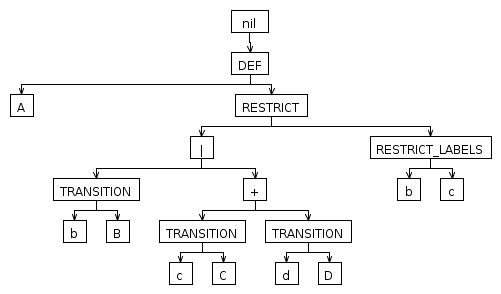
\includegraphics[width=3.5in]{ast_example}
\caption{Abstract syntaxt tree example}
\label{fig:ast_example}
\end{figure}

\subsection{CCS domain model and labeled graph generation}
Although working directly with abstract syntax trees and performing all algorithms on them is possible, it causes 
a limitation in future changes, where even a small change in the grammar and/or in the structure of the
generated abstract syntax trees causes a change in the implemented algorithms. Because of this,
a specific domain model is built along with a domain builder algorithm, which has corresponding
abstractions for all CCS operators, processes and actions. The input of the domain builder algorithm 
is an abstract syntax tree, and the output is a fully built domain model. The algorithms for constructing a labeled graph 
are implemented on the domain model because it is not expected for the domain model structure to 
change much in the future. The domain model is also a tree-like structure, so it is as easy to work with, 
as with the abstract syntax tree. 

The algorithm for generation of labeled transition system is a recursive algorithm which traverses the tree structure of objects 
in the domain model and performs SOS rule every time it reaches an operation.
In this fashion all SOS transformation are performed on the domain and as result a new graph
structure is created which represents the labeled transition system which can be easily exported to a file
in Aldebaran format.

\subsection{Workflow of operations}
In  Fig. \ref{fig:workflow} the workflow of all operations that are executed for constructing a labeled transition system graph from a 
CCS expression are shown. Every operation is done as a standalone algorithm independent from the other operations,
that has input and output shown in the figure. The modular design is deliberately chosen in order to help achieve better 
testing and maintenance of the source code. 

\begin{figure}[h]
\centering
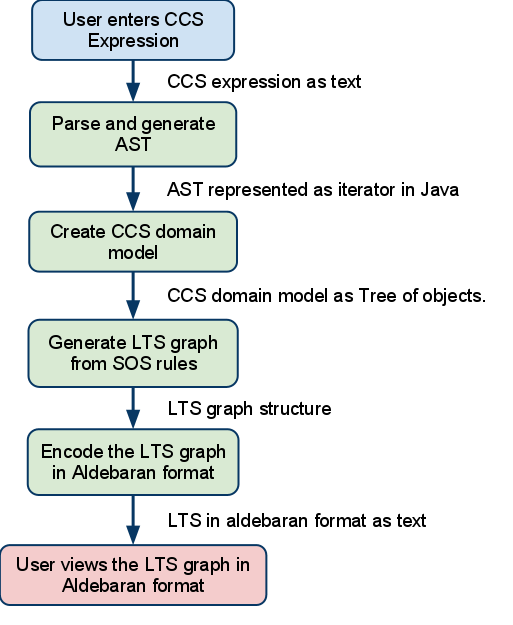
\includegraphics[height=3.0in]{workflow}
\caption{Workflow of all operations for producing a labeled transition system graph from a CCS expression}
\label{fig:workflow}
\end{figure}
 % Chapter2
\section{Bisimulation equivalence}
% no \IEEEPARstart
Bisimulation equivalence (bisimilarity)\footnote{The notion of bisimulation equivalence (bisimilarity) in this chapter 
refers to strong bisimulation equivalence (strong bisimilarity)} is a binary relation between labeled transition systems which associates systems that can simulate each other's behaviour in a stepwise manner. This enables comparison of different transition systems. An alternative perspective is to consider bisimulation equivalence as a relation between states of a single labelled transition system. By considering the quotient transition system under such a relation, smaller models are obtained \cite{ModelChecking}.

The bisimulation equivalence finds its extensive application in many areas of computer science such as concurrency theory, formal verification, set theory, etc. For instance, in formal verification minimization with respect to bisimulation equivalence is used to reduce the size of the state space to be analyzed. Also, bisimulation equivalence is of particular interest in model checking, in specific to check the equivalence of an implementation of a certain system with respect to its specification model.

Our tool implements both options: reducing the size of the state space of a given LTS (minimization modulo bisimilarity) and checking the equivalence of two labeled transition systems modulo bisimilarity.

\subsubsection{Minimization of an LTS modulo bisimilarity.}
The process of reducing the size of the state space of a certain labeled transition system was implemented using an approach which consists of two steps:
\begin{enumerate}
\item Computing strong bisimulation equivalence (strong bisimilarity) for the LTS;
\item Minimizing the LTS to its canonical form using the strong bisimilarity obtained in the first step;
\end{enumerate}

The first step, computing strong bisimulation equivalence, was implemented with two different methods: the so called
naive method and a more efficient method due to Fernandez, both of which can serve as minimization procedures.

The naive algorithm \cite{ReactiveSystems1} for computing bisimulation equivalence stems from the theory underlying 
Tarski's fixed point theorem \cite{ReactiveSystems2}. It has been proven that the strong bisimulation equivalence is 
the largest fixed point of the monotic function $F$ as defined in \cite{ReactiveSystems1} given by Tarsky's fixed 
point theorem. 

The labeled graph was represented as a list of nodes and the following terminology was used:
\begin{itemize}
	\item $S_p=\{(a, q)\}$ - set of pairs $(a, q)$ for state $p$ where $a$ is an outgoing action for $p$ and $q$ is a state
	reachable from $p$ with the action $a$
\end{itemize}

Our Java implementation of the algorithm takes as input an LTS in aldebaran format, generates a corresponding labeled 
graph and then computes the strong bisimulation equivalence as pairs of bisimilar states.

This algorithm has time complexity of $O(mn)$ for a labeled transition system with \emph{m} transitions and \emph{n} 
states. 

The algorithm due to Fernandez exploits the idea of the relationship between strong bisimulation equivalence 
and the relational coarsest partition problem solved by Paige and Tarjan. It represents adaptation of the 
Paige-Tarjan algorithm of complexity $O(m \log n)$ to minimize labeled transition systems modulo bisimulation 
equivalence by computing the coarsest partition problem with respect to the family of binary relations 
$\left(T_a\right)_{a\in A}$ instead of one binary relation, where $T_a=\{(p,q)|(p,a,q)\in T\}$ is a transition 
relation for action $a\in A$ and $T$ is a set of all transitions \cite{PaigeTarjan}\cite{Fernandez}.

The algorithm due to Fernandez in our Java implementation takes an LTS in aldebaran format as an input, generates a 
corresponding labeled graph and then partitions the labeled graph into its coarsest blocks where each block represents 
a set of bisimilar states. Partition is a set of mutually exclusive blocks whose union constitutes the graph universe.

To define graph transitions the following terminology was used: 
\begin{itemize}
	\item $T_a[p]=\{q\}$ - an $a$-transition from state $p$ to state $q$
	\item $T_a{}^{-1}[q]=\{p\}$ - an inverse $a$-transition from state $q$ to state $p$
	\item $T_a{}^{-1}[B]=\cup \left\{T_a{}^{-1}[q],q\in B\right\}$ - inverse transition for block $B$ and action $a$
	\item $W$ - set of sets called splitters that are being used to split the partition
	\item infoB$(a, p)$ - info map for block $B$, state $p$ and action $a$
\end{itemize}

The time complexity of Fernandez's algorithm is $O(m \log n)$ for a labeled transition system 
with $m$ transitions and $n$ states. 

The next step in the reduction of the state space of an LTS uses the bisimulation equivalence computed in the first step in order to minimize the labeled graph. This reduction is implemented as follows:
\begin{enumerate}
	\item If a pair of states $(p, q)$ is bisimilar, then the two states are merged into one single state $k$;
	\item All incoming transitions $r \stackrel{a}{\rightarrow} p$ and $s \stackrel{a}{\rightarrow} q$ are replaced by transitions $r \stackrel{a}{\rightarrow} k$ and $s \stackrel{a}{\rightarrow} k$;
	\item All outgoing transitions $p \stackrel{a}{\rightarrow} r$ and $q \stackrel{a}{\rightarrow} s$ are replaced by transitions $k \stackrel{a}{\rightarrow} r$ and $k \stackrel{a}{\rightarrow} s$;
	\item The duplicate transitions are not taken into consideration.
\end{enumerate}
The procedure is repeated for all pairs of bisimilar states.

The process of reducing a given labeled graph module strong bisimilarity is illustrated below for the labeled graph in Fig. \ref{fig:graph1}.

\begin{figure}[!ht]
\centering
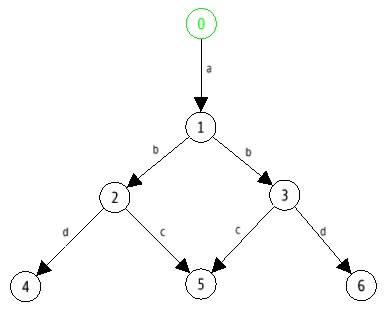
\includegraphics[width=2.3in]{graph1}
\caption{Graph 1}
\label{fig:graph1}
\end{figure}

Applying both the naive and the advanced algorithm due to Fernandez for computing strong bisimulation equivalence for Graph 1, gives the results shown in Table \ref{table1}.
\begin{table}[!ht]
\begin{tabular}{| l | p{10.5cm}| }
  \hline                       
  Algorithm & Graph 1 \\ \hline
  Naive & (2, 3), (3, 2), (4, 5), 
(5, 4), (4, 6), (6, 4), (5, 6), (6, 5), (0, 0), (1, 1), (2, 2), (3, 3), (4, 4), (5, 5), (6, 6) \\ \hline
  Fernandez & \{0\}, \{1\}, \{2\}, \{3\}, \{4, 5, 6\} \\ \hline  
\end{tabular}
\\
\caption{Computing strong bisimularity for Graph 1}
\label{table1}
\end{table}

The results obtained with either of the two algorithms for computing strong bisimilarity are then used as a basis for the reduction of the given graph to its minimal form. Namely, all mutually bisimilar states are merged into a single state and their transitions are updated accordingly. The reduction of Graph 1 to its canonical form with respect to the bisimulation equivalence is given in Fig.  \ref{fig:bisimGraph1}. As it can be seen from the figure, the states 2 and 3 are merged into state 2 in the minimal graph, and states 4, 5 and 6 are merged into state 3 in the minimal graph.

\begin{figure}[!ht]
\centering
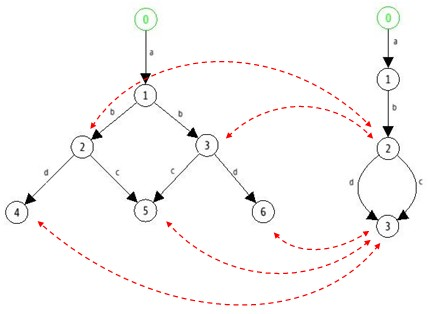
\includegraphics[width=2.8in]{bisimGraph1}.
\caption{Minimized Graph 1}
\label{fig:bisimGraph1}
\end{figure}

\subsubsection{Comparison of two LTSs modulo bisimilarity.}
The idea for the implementation of the equivalence checking of two labeled transition systems modulo strong bisimilarity was based on the following fact: Two labelled transition systems are (strongly) bisimilar iff their initial states are bisimilar \cite{ModellingAndAnalysis}.

That means that in order to check whether two labeled transition systems are bisimilar it is enough to check whether their initial states are bisimilar. This can be done using the following approach:
\begin{enumerate}
	\item The two labeled transition systems are merged into a single transition system
	\item An algorithm for computing the strong bisimilarity is applied to the merged system
	\item A check is performed to see if the initial states belong to the same bisimulation equivalence class
\end{enumerate}

The correctness of the implementation was tested with the use of ltsconvert and ltscompare tools of mCRL2, micro Common Representation Language 2, a specification language that can be used to specify and analyse the behaviour of distributed systems and protocols
\cite{mCRL2Ref}.
 % Chapter3
\section{Saturation and weak bisimulation equivalence}
% no \IEEEPARstart
Def: Let $P$ and $Q$ be CCS processes or, more generally, states in a labeled transition system. For each action $a$, we shall write
$P\stackrel{a}{\Rightarrow}Q$ iff:
\begin{itemize}
	\item Either $a\neq\tau$ and there are processes $P'$ and $Q'$ such that $P\left(\stackrel{\tau}{\rightarrow}\right)^{*}P'\ \stackrel{a}{\rightarrow}\ Q'\left(\stackrel{\tau}{\rightarrow}\right)^{*}Q$,
	\item Or $a=\tau$ and $P\left(\stackrel{\tau}{\rightarrow}\right)^{*}Q$,
\end{itemize}
where we write $\left(\stackrel{\tau}{\rightarrow}\right)^{*}$ for he reflexive and transitive closure of the relation $\stackrel{\tau}{\rightarrow}$.

Def: (weak bisimulation and observational equivalence) A binary relation $R$ over the set of states of an LTS is a weak bisimulation iff, whenever $s_{1}Rs_{2}$ and $a$ is an action (including $\tau$):
\begin{itemize}
	\item If $s_{1}\stackrel{a}{\rightarrow}s_{1}'$ then there is a transition $s_{2}\stackrel{a}{\Rightarrow}s_{2}'$ such that $s_{1}'Rs_{2}'$;
	\item If $s_{2}\stackrel{a}{\rightarrow}s_{2}'$ then there is a transition $s_{1}\stackrel{a}{\Rightarrow}s_{1}'$ such that $s_{1}'Rs_{2}'$;
\end{itemize}

Two states $s$ and $s'$ are observationally equivalent (or weakly bisimilar), written $s\approx s'$, iff there is a weak bisimulation equivalence that relates them.

Def: Let $T\subseteq S\times Act\times S$ be an LTS. We shall say that\\ 
$T^{*}=\left\{\left(p,a,q\right)| p\stackrel{a}{\Rightarrow}q\right\}=T\cup\left(\stackrel{a}{\rightarrow}\right)^{*}\cup\left\{\left(p,a,q\right)| a\neq\tau\wedge\left(\exists p',q'\in A\right) p\left(\stackrel{\tau}{\rightarrow}\right)^{*}p'\stackrel{a}{\rightarrow}q'\left(\stackrel{\tau}{\rightarrow}\right)^{*}q\right\}$ is a saturation of T.

Proposition: Two LTSs are weakly bisimilar iff their saturated LTSs are strongly bisimilar. 

Proof: Let $T$ and $U$ be two LTSs for which their saturated LTSs are strongly bisimilar by the relation $R$. Since the strong bisimulation is also a weak bisimulation it follows that $T$ and $U$ are weakly bisimular, since they are weakly bisimular to their respective saturated LTSs.
Let $T$ and $U$ be two LTSs that are weakly bisimilar. Let $u\approx t$, $u'\approx t'$. If $t\stackrel{a}{\rightarrow}t'\in T^{*}$, that means $t\stackrel{a}{\Rightarrow}t'$, or that there exist states $t_{i}$, $t'_{j}$ such that: $t\stackrel{\tau}{\rightarrow}t_{1}\stackrel{\tau}{\rightarrow}...\stackrel{\tau}{\rightarrow}t_{k}\stackrel{a}{\rightarrow}t'_{1}\stackrel{\tau}{\rightarrow}...\stackrel{\tau}{\rightarrow}t'_{m}\stackrel{\tau}{\rightarrow}t'$. Let $u_{i}\approx t_{i}$,...,$u'_{j}\approx t'_{j}$,.... It follows that $u\stackrel{\tau}{\Rightarrow}u_{1}\stackrel{\tau}{\Rightarrow}...\stackrel{\tau}{\Rightarrow}u_{k}\stackrel{a}{\Rightarrow}u'_{1}\stackrel{\tau}{\Rightarrow}...\stackrel{\tau}{\Rightarrow}u'$, or that there exist states $u''$, $u'''$ in U such that $u\left(\stackrel{\tau}{\rightarrow}\right)^{*}u_{k}\left(\stackrel{\tau}{\rightarrow}\right)^{*}u''\stackrel{a}{\rightarrow}u'''\left(\stackrel{\tau}{\rightarrow}\right)^{*}u'_{1}\left(\stackrel{\tau}{\rightarrow}\right)^{*}u'$ which means $u\stackrel{a}{\Rightarrow}u'$. Since $U^{*}$ is a saturation of $U$, it follows that $u\stackrel{a}{\rightarrow}u'\in U^{*}$.
Similarly, for every transition $u\stackrel{a}{\rightarrow}u'\in U^{*}$, there is a transition in $t\stackrel{a}{\rightarrow}t'\in T^{*}$, such that $u\approx t$, $u'\approx t'$.
Therefore, the weak bisimulation relation $\approx$ for $T$ and $U$ is a strong bisimulation relation for $T^{*}$ and $U^{*}$.

\subsection{The algorithm for saturation.}

The set of triples ${R}$ can be partitioned in ${2n}$ sets with: \\
\ \ \ \ ${T_{\tau p}=\left\{\left(p,\tau,q\right)| \left(p,\tau,q\right)\in T\right\}}$, and\\
\ \ \ \ ${T_{ap}=\left\{\left(p,\tau,q\right)|\ a\neq\tau\wedge\left(p,\tau,q\right)\in T\right\}}$ for every ${p\in S}$.

By the definition of ${T_{\tau p}}$ and ${T_{ap}}$ it can be seen that ${\bigcup_{p\in S}\left(T_{\tau p}\cup T_{ap}\right)=T}$, and also, their pairwise intersection is empty. 

The family of sets ${T^{*}_{\tau p}}$ can be iteratively constructed with:\\
${T^{0}_{\tau p}=T_{\tau p}\cup\left\{\left(p,\tau,p\right)\right\}}$,\\
${T^{i}_{\tau p}=T^{i-1}_{\tau p}\cup\left\{\left(p,\tau,r\right)|\left(\exists q\in S\right)\left(p,\tau,q\right)\in T^{i-1}_{\tau p}\wedge\left(q,\tau,r\right)\in T_{\tau q}\right\}}$ and \\
${T^{*}_{\tau p}=T^{n}_{\tau p}}$

(Note: ${\left|T^{*}_{\tau p}\right|\leq\left|S\right|=n}$; when for some ${k<n}$, ${T^{k}_{\tau p}=T^{k+1}_{\tau p}}$, then ${T^{*}_{\tau p}=T^{k}_{\tau p}=T^{n}_{\tau p}}$)

With this step a reflexive, transitive closure was constructed: ${T^{*}_{\tau}=\bigcup_{p\in A}T^{*}_{\tau p}=\left\{\left(p,\tau,q\right)|p\left(\stackrel{\tau}{\rightarrow}\right)^{*}q\right\}}$.

\begin{figure}[!ht]
\centering
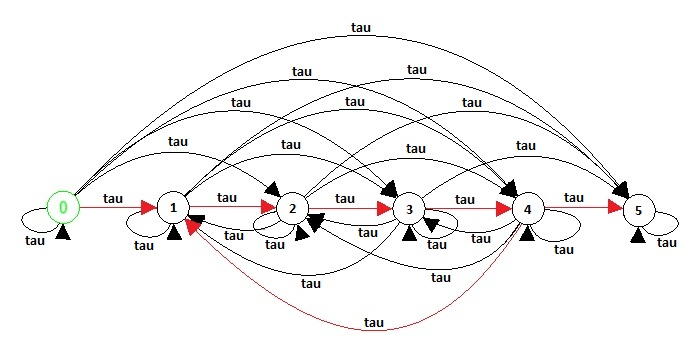
\includegraphics[width=4.5in]{saturation}
\caption{Reflexive, transitive closure of $\tau$. The original graph is depicted with red lines}
\label{fig:saturation}
\end{figure}

The next step is to construct $T'_{ap}=\bigcup_{p\in A}T'_{ap}=\left\{\left(p,a,q\right)|\left(\exists q'\in S\right)\left(p,a,q'\right)\in T\wedge q'\left(\stackrel{\tau}{\rightarrow}\right)^{*}q\right\}$:\\
$T^{0}_{ap}=T_{ap'}$,\\
$T^{i}_{ap}=T^{i-1}_{ap}\cup \left\{\left(p,a,r\right)|\left(\exists q\in S\right)\left(p,a,q\right)\in T^{i-1}_{ap}\wedge \left(q,\tau,r\right)\in T^{i-1}_{\tau q}\right\}$ and \\
$T'_{ap}=T^{n|Act|}_{ap}$

(Note: $|T'_{ap}|\leq |S||Act|=n|Act|$, when for some $k<n|Act|$, $T^{k}_{ap}=T^{k+1}_{ap}$, then $T'_{ap}=T^{k}_{ap}=T^{n|Act|}_{ap}$)

For the third step, $T'=\bigcup_{p\in S}\left(T^{*}_{\tau p}\cup T'_{ap}\right)$ needs to be partitioned again, defined by the destination in the triple:\\
$T_{\tau q}=\left\{\left(p,\tau,q\right)|\left(p,\tau,q\right)\in T'\right\}$ and $T_{bq}=\left\{\left(p,a,q\right)|a\neq\tau\wedge\left(p,a,q\right)\in T'\right\}$ for every $p\in S$,\\
and then construct:\\
$T^{0}_{bq}=T_{bq}$,\\
$T^{i}_{bq}=T^{i-1}_{bq}\cup\left\{\left(p',a,q\right)|\left(\exists p\in S\right)\left(p,a,q\right)\in T^{i-1}_{bq}\wedge\left(p',\tau,p\right)\in T^{*}_{\tau p}\right\}$ and\\
$T^{*}_{bq}=T^{n|Act|}_{bq}$

Finally the saturated LTS is:\\
$T^{*}=\bigcup_{p\in S}\left(T^{*}_{\tau p}\cup T^{*}_{bp}\right)=\left(\stackrel{\tau}{\rightarrow}\right)^{*}\cup\left\{\left(p,a,q\right)|a\neq\tau\wedge\left(\exists p',q'\in A\right) p\left(\stackrel{\tau}{\rightarrow}\right)^{*}p'\stackrel{a}{\rightarrow}q'\left(\stackrel{\tau}{\rightarrow}\right)^{*}q\right\}$

\begin{figure}[!ht]
\centering
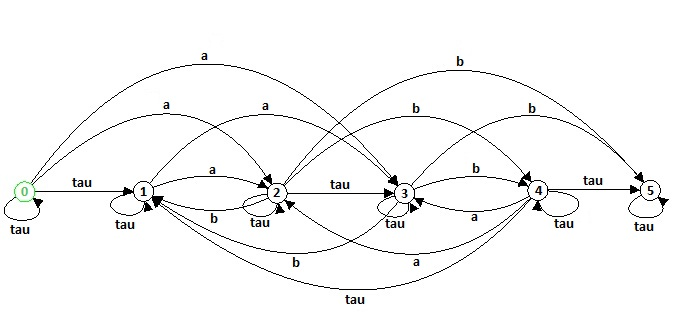
\includegraphics[width=4.5in]{saturation2}
\caption{Example saturated LTS}
\label{fig:saturation2}
\end{figure} % Chapter4
\section{Alternating Bit Protocol - modelling, specification and testing}
% no \IEEEPARstart
The alternating bit protocol is a simple yet effective protocol (usually used as a test case), designed to ensure reliable communication through unreliable transmission mediums, and it�s used for managing the retransmission of lost messages \cite{ReactiveSystems3}\cite{Kulick}.

The representation of Alternating Bit Protocol is shown bellow, and it consists of $Sender$ $S$, $Receiver$ $R$ and two channels $Transport$ $T$ and $Acknowledge$ $A$. In the following text Alternating Bit Protocol is abbreviated as ABP.

\begin{figure}[!ht]
\centering
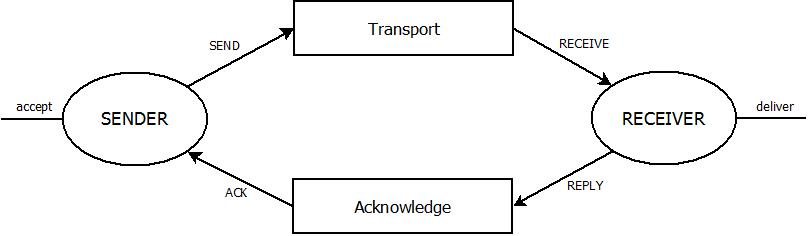
\includegraphics[width=4.5in]{abp}
\caption{Alternating bit protocol}
\label{fig:abp}
\end{figure}

All of the transitions in the ABP are internal synchronization and the only visible transitions are deliver and accept, which can occur only sequentially. 

Here is the specification of ABP:\\
$ABP=\overline{deliver}.accept.ABP$

Messages are sent from a sender $S$ to a receiver $R$. Channel from $S$ to $R$ is initialized and there are no messages in transit. There is no direct communication between the sender $S$ and the receiver $R$, and all messages must travel trough the medium (transport and acknowledge channel). The ABP works like this:
\begin{enumerate}
	\item Each message sent by $S$ contains the protocol bit, 0 or 1.\\
	      Here is the implementation:\\
	      $Imp=\left(S|T|R|A\right)\backslash\left{send0,send1,receive0,receive1,reply0,reply1,ack0,ack1\right}$
	\item When a sender $S$ sends a message, it sends it repeatedly (with its corresponding bit) until receiving an acknowledgment ($ack0$ or $ack1$) from a receiver $R$ that contains the same protocol bit as the message being sent.\\
	      $S=\overline{send0}.S+ack0.accept.S_{1}+ack1.S$\\
	      $S_{1}=\overline{send1}.S_{1}+ack1.accept.S+ack0.S_{1}$\\
	      The transport channel transmits the message to the receiver, but it may lose the message (lossy channel) or transmit it several times (chatty channel).
	      $T=send0.\left(T+T_{1}\right)+send1.left(T+T_{2}\right)$\\
	      $T_{1}=\overline{receive0}.\left(T+T_{1}\right)$\\
	      $T_{2}=\overline{receive1}.\left(T+T_{2}\right)$
  \item When $R$ receives a message, it sends a reply to $S$ that includes the protocol bit of the message received. When a message is received for the first time, the receiver delivers it for processing, while subsequent messages with the same bit are simply acknowledged.
        $R=receive0.\overline{deliver}.R_{1}+\overline{reply1}.R+receive1.R$\\
        $R_{1}=receive1.\overline{deliver}.R+\overline{reply0}.R_{1}+receive0.R_{1}$\\
        Again the acknowledgement channel sends the ack to sender, and it also can acknowledge it several times or lose it on the way to the sender.\\
        $A=reply0.\left(A+A_{1}\right)+reply1.\left(A+A_{2}\right)$\\
        $A_{1}=\overline{ack0}.\left(A+A_{1}\right)$\\
        $A_{2}=\overline{ack1}.\left(A+A_{2}\right)$
  \item When $S$ receives an acknowledgment containing the same bit as the message it is currently transmitting, it stops transmitting that message, flips the protocol bit, and repeats the protocol for the next message.\cite{Kulick}\cite{ProcessAlgebraParallel}
\end{enumerate}
 % Chapter5
\section{Peterson and Hamilton algorithm - Modeling,  Specification and Testing}
% no \IEEEPARstart
The algorithm

var flag: array [0..1] of boolean; 
turn: 0..1; 
%flag[k] means that process[k] is interested in the critical section 
flag[0] := FALSE; 
flag[1] := FALSE; 
turn := random(0..1) 

%After initialization, each process, which is called process i in the code, runs this code: 

repeat 
flag[i] := TRUE; 
turn := j; 
while (flag[j] and turn=j) do no-op; 
%CRITICAL SECTION 
flag[i] := FALSE; 
%REMAINDER SECTION 
until FALSE;

There are two different processes which want to enter at critical section. 
This means that the processes are fighting for one resource (ex. Say one variable or data structure). 
flag[i]= true means that process I wants to enter the critical section and the turn=i means that process i is next to enter the critical section.
 At first the shared variables flag[0] and flag[1] are initialized to false because neither process is yet interested in the critical section. 
 The shared variable turn is set to either 0 or 1 randomly (or it can always be set to say 0). 
 If the process can’t enter the critical section it waits in while loop.

Legend:

turn € {0, 1}
flag0, flag1 € {true, false} = {t, f}

w – write
r – read
enter – enter the critical section
exit – exit the critical section

Initialization:

turn=1
flag1 = flag2 = f

CCS Specification:

Peterson = (P1 | P2 | flag1f | flag2f | turn1) \ L

P1 = flag1wt.turnw2.P11
P11 = flag2rf.P12 + flag2rt.(turnr2. τ.P11 + turnr1.P12)
P12 = enter1.exit1.flag1wf.P1

P2 = flag2wt.turnw1.P21
P21 = flag1rf.P22 + flag1rt.(turnr1. τ.P21 + turnr2.P22)
P22 = enter2.exit2.flag2wf.P2

FLAG1f = flag1rf.flag1f + flag1wf.flag1f + flag1wt.flag1t
FLAG1t = flag1rt.flag1t + flag1wt.flag1t + flag1wf.flag1f

FLAG2f = flag2rf.flag2f + flag2wf.flag2f + flag2wt.flag2t
FLAG2t = flag2rt.flag2t + flag2wt.flag2t + flag2wf.flag2f

TURN1 = turnr1.turn1 + turnw1.turn1 + turnw2.turn2
TURN2 = turnr2.turn2 + turnw2.turn2 + turnw1.turn1

L = { flag1wt, flag1rt, turnw2,… union of the access sorts (r,w) of the
variables }

\begin{figure}[!t]
\centering
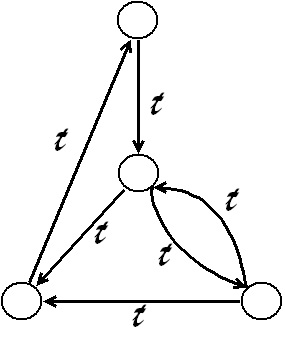
\includegraphics[width=3.5in]{model1}
% where an .eps filename suffix will be assumed under latex, 
% and a .pdf suffix will be assumed for pdflatex; or what has been declared
% via \DeclareGraphicsExtensions.
\caption{AST Example}
\label{fig:ast_example}
\end{figure}

\begin{figure}[!t]
\centering
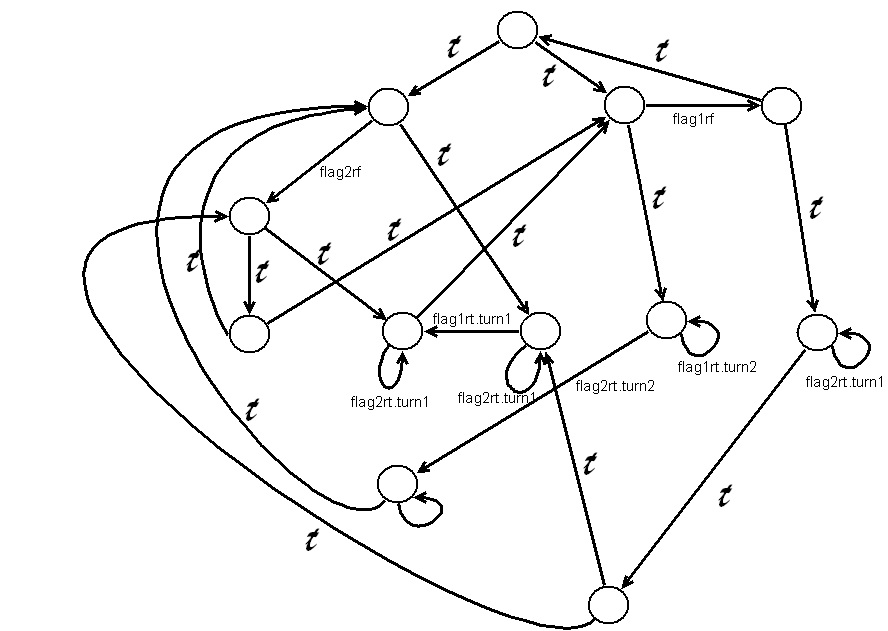
\includegraphics[width=3.5in]{model2}
% where an .eps filename suffix will be assumed under latex, 
% and a .pdf suffix will be assumed for pdflatex; or what has been declared
% via \DeclareGraphicsExtensions.
\caption{AST Example}
\label{fig:ast_example}
\end{figure}

The mutual exclusion requirement is assured. Suppose instead that both processes are in their critical section. 
Only one can have the turn, so the other must have reached the while test before the process with the turn set its flag. 
But after setting its flag, the other process had to give away the turn. 
Contradicting our assumption, the process at the while test has already changed the turn and will not change it again.
	The progress requirement is assured. 
	Again, the turn variable is only considered when both processes are using, or trying to use, the resource.
	Deadlock is not possible. One of the processes must have the turn if both processes are testing the while condition. 
	That process will proceed.
	Finally, bounded waiting is assured. When a process that has exited the CS reenters, it will give away the turn. 
	If the other process is already waiting, it will be the next to proceed.

Test and set algorithm

repeat
while Test-and-Set(lock) do no-op;
critical section 
lock := false;
remainder section 
until false 

Test-and-Set(target) 
result := target;
target := true; 
return result 

\begin{tabular}{ | l | l | }
  \hline                       
  Process 1	& Process 2 \\ \hline 
  Wants to set target to true & \\
  Target is changed to true & \\
  Result comes back false so no busy waiting &\\
  & Wants to set target to true \\
  & It receives the result true \\
  & Busy waits as long as Process 1 is in critical section \\
  Leaves critical section & \\
  Set target to false & \\
  \hline  
\end{tabular}
 % Chapter6
\section{HML and $U^{w}$ and $U^{s}$ operators}
\label{sec:hml}

Henessy-Milner logic \cite{HenessyMilner} is a multimodal logic used to characterize the properties of a system which describe some aspects of the system's behaviour. Its syntax is defined by the following BNF grammar \cite{ModelingAndAnalysis}:
\begin{equation}\label{eq:hml_bnf}
\phi ::= \mathit{tt} \hspace{1 mm} | \hspace{1 mm} \mathit{ff} \hspace{1 mm} | \hspace{1 mm} \neg\phi \hspace{1 mm} | \hspace{1 mm}\phi\wedge\phi \hspace{1 mm} |
\hspace{1 mm} \phi\vee\phi | \left\langle a\right\rangle \phi \hspace{1 mm} | \hspace{1 mm} \left[a\right]\phi \hspace{1 mm}
\end{equation}

A single HML formula can only describe a finite part of the overall behavious of a process. Therefore, the Henessy-Milner logic was extended to allow for recursive definitions by the introduction of two operators: the so called 'strong until' operator $U^{s}$ and the so called 'weak until' operator $U^{w}$. These operators are expressed as follows \cite{ReactiveSystems}:

\begin{equation}
	\begin{array}{lcl}
		F \hspace{1 mm} U^{s} \hspace{1 mm} G \stackrel{min}{=} G \vee \left(F \wedge \langle Act \rangle tt \wedge \left[Act\right]\left(F \hspace{1 mm} U^{s} \hspace{1 mm} G\right)\right)\\
		F \hspace{1 mm} U^{w} \hspace{1 mm} G \stackrel{max}{=} G \vee \left(F \wedge \left[Act\right] \left(F \hspace{1 mm} U^{w} \hspace{1 mm} G\right)\right)
	\end{array}
\end{equation}

The BNF grammar describing the set of HML formulas with recursion is as follows \cite{HMLRecursion}:

\begin{equation}\label{eq:hmlrec_bnf}
\phi ::= tt \hspace{1 mm} | \hspace{1 mm} ff \hspace{1 mm} | \hspace{1 mm} \neg\phi \hspace{1 mm} | \hspace{1 mm}\phi\wedge\phi \hspace{1 mm} |
\hspace{1 mm} \phi\vee\phi | \left\langle a\right\rangle \phi \hspace{1 mm} | \hspace{1 mm} \left[a\right]\phi \hspace{1 mm} | \hspace{1 mm} X | \hspace{1 mm} min\left(X,\phi \right) \hspace{1 mm} | \hspace{1 mm} max\left(X,\phi \right) \hspace{1 mm}
\end{equation}
where $X$ is a formula variable and $min\left(X,\phi\right) \hspace{1 mm}$ (respectively $max\left(X,\phi\right) \hspace{1 mm}$) stands for the least (respectively largest) solution of the recursion equation $X = \phi$.

\subsection{HML parsing}
Our implementation of the Hennessy-Milner logic works as follows: For a given HML expression and a labeled transition system, we should get an output whether that expression is valid for the corresponding labeled graph. One HML expression can be made of these set of tokens \{"AND", "OR", "UW", "US", "NOT", "[", "]", "$\langle$", "$\rangle$", "TT", "FF", "(", ")", "$\{$", "$\}$", ","\}

The first part of this process is called tokenization. Tokenization is the process of demarcating and possibly classifying sections of a string of input characters. The resulting tokens are then passed on to some other form of processing.

The process can be considered as a sub-task of parsing input. As the tokens are being read they are proceeded to the parser. The parser is a LR top-down parser. This parser is able to recognize a non-deterministic grammar which is essential for the evaluation of the Hennessy-Milner expression. As the parser is reading the tokens, thus in a way we “move” through the graph and determine if some of the following steps are possible. Every condition is in a way kept on stack and that enables later return to any of the previous conditions. The process is finished when the expression is processed or when it is in a condition from which none of the following actions can be taken over.

\subsection{$U^{w}$ and $U^{s}$ implementation}
The implementation of the $U^{w}$ and $U^{s}$ operators was done as follows. First we get the current state which is the state that contains all the nodes that satisfied the previous actions. For example if we have expression 
\begin{equation*}
	\langle a\rangle\langle a\rangle TT \hspace{1 mm} U^{s} \hspace{1 mm} \langle b\rangle TT, 
\end{equation*}
then we get all the nodes that we can reach, starting from the start node, with two actions “a”. When we get to the “Until” operation, in this case $U^{s}$, we take the start state and check if we can make an action $b$ from some node. If we cannot do the action $b$, then we repeat the process, do action $a$ again and check if can we do action $b$. This process is being repeated until we come to a state in which we can't do action a from all nodes in that state.

In the end we check the operator's type (strong or weak). If the operator is strong, then only one node in its state is enough. If it is weak, we check if there are no nodes in its new state or if we can get from the starting node to some of its neighbors through the action $b$. 

 % Chapter7
\section{Conclusions and Future Work}
\label{sec:conclusion}

In this paper we presented a tool for modeling, manipulation and analysis of concurrent systems. It includes recognizing CCS expressions, building labeled transition system graphs and checking equivalence between two labeled graphs with respect to strong and weak bisimilarity. The tool is very simple, but yet functional enough to perform specification and verification of concurrent systems described as CCS expressions and/or labeled transition systems graphs. We have successfully tested the tool with large number of examples comparing the results obtained with mCRL2 and CWB, and we also presented few examples showing the tool usage. 

Future work can include optimization of the tool response times for very large labeled transition system graphs, as well as implementation of prunung strategy for infinite labeled transition system graphs. It would be also usefull if the labeled graph is better visualized where every SOS rule is shown, with its source and sink nodes showing the CCS expression for each of the nodes. Such a visualization can be very helpfull for understanding the semantics of the CCS language for students that are starting to study it. Furthermore, the minimization and comparison functionality for labeled transition systems which at the moment includes only strong and weak bisimilarity can be extended to include other behavioural equivalences as well. Another direction for future development can be to extend the tool to support not only CCS expressions, but variety of other process semantics as well. 
 % Chapter9
% use section* for acknowledgement
\section*{Acknowledgment}


The authors would like to thank Jasen Markovski for being their mentor... 
% references section

\begin{thebibliography}{[1]}
%\bibstyle{splncs}

\bibitem{Milner1}
R. Milner,
\emph{A Calculus of Communicating Systems},
Lecture Notes in Computer Science, vol. 92, Springer-Verlag, 1980

\bibitem{Milner2}
R. Milner,
\emph{Communication and Concurrency},
Prentice-Hall, 1989

\bibitem{HandbookProcessAlgebra}
J.A. Bergstra, A. Ponse, S.A. Smolka, 
\emph{Handbook of Process Algebra}, 
Elsevier Science B.V., 2001

\bibitem{Keller}
R.M. Keller,
\emph{Formal Verification of Parallel Programs},
Communications of the ACM, 19(7), pp. 371-384, 1976

\bibitem{ReactiveSystems}
L. Aceto, A. Ingolfsdottir, K. G. Larsen, J. Srba,
\emph{Reactive Systems - Modeling, Specification and Verification},
Cambridge University Press, 2007

\bibitem{Park}
D.M.R. Park,
\emph{Concurrency and Automata on Infinite Sequences},
In: Proceedings of the 5th G.I.Conference in Theoretical Computer Science, 
Lecture Notes in Computer Science, vol. 104, Springer-Verlag, pp. 167-183, 1981

\bibitem{UnderstandingConcurrentSystems}
A.W. Roscoe,
\emph{Understanding Concurrent Systems},
Texts in Computer Science, Springer-Verlag, 2010

\bibitem{Milner3}
R. Milner,
\emph{Operational and Algebraic Semantics of Concurrency Processes},
In: J. van Leeuwen (ed.) Handbook of Theoretical Computer Science, pp. 1201-1242,
Elsevier and MIT Press, 1990

\bibitem{ModelChecking}
C. Baier, J.-P. Katoen, 
\emph{Principles of Model Checking},
The MIT Press, 2008

\bibitem{HennessyMilner}
M.C.B. Hennessy, R. Milner,
\emph{Algebraic Laws for Nondeterminism and Concurrency},
Journal of the ACM, 32(1), pp. 137-161, 1985

\bibitem{Larsen}
K.G. Larsen,
\emph{Proof Systems for satisfiability in Hennessy�Milner logic with recursion}, 
Theoretical Computer Sciece, 72(2-3), Special Issue, pp. 265�288, 1990

\bibitem{Jar}
The Java tutorials,
\emph{Packaging Programs in JAR Files},
\url{http://download.oracle.com/javase/tutorial/deployment/jar/index.html}

\bibitem{Aldebaran}
CADP manual, 
\emph{Aldebaran format for Labeled Transition Systems},
\url{http://www.inrialpes.fr/vasy/cadp/man/aldebaran.html#sect6}

\bibitem{CWB}
\emph{The Edinburgh Concurrency Workbench (CWB)},	
\url{http://homepages.inf.ed.ac.uk/perdita/cwb/summary.html}

\bibitem{mCRL2}
\emph{micro Common Representation Language 2 (mCRL2)},	
\url{http://www.mcrl2.org}

\bibitem{MWB}
\emph{The Mobility Workbench (MWB)},
\url{http://www.it.uu.se/research/group/mobility/mwb}

\bibitem{CADP}
\emph{Construction and Analysis of Distributed Processes (CADP)},
\url{http://www.inrialpes.fr/vasy/cadp.html}

\bibitem{LTSA}
\emph{Labelled Transition System Analyser (LTSA)},
\url{http://www.doc.ic.ac.uk/ltsa/}

\bibitem{Fernandez}
J.-C. Fernandez, 
\emph{An Implementation of an Efficient Algorithm for Bisimulation
Equivalence}, Science of Computer Programming, vol. 13, pages 219-236, 1989/1990

\bibitem{ABP1}
W.C. Lynch, 
\emph{Computer systems: Reliable full-duplex file transmission over half-duplex telephone line},
Communications of the ACM, vol. 11, no. 6, pp. 407�410, 1968

\bibitem{ABP2}
K.A. Bartlett, R.A. Scantlebury, P.T. Wilkinson, 
\emph{A note on Reliable Full-duplex Transmission over Half-duplex Links},
Communications of the ACM, vol. 12, pp. 260�261, 1969

\bibitem{Peterson}
G.L. Peterson,
\emph{Myths about the Mutual Exclusion Problem}, 
Information Processing Letters, 12(3), pages 115-116, 1981

\bibitem{ModellingAndAnalysis}
J.F. Groote, M. Reniers, 
\emph{Modelling and Analysis of Communicating Systems}\emph, 
Technical University of Eindhoven, rev. 1478, 2009

\bibitem{Chomsky}
N. Chomsky,
\emph{Three Models for the Description of Language},
IEEE Transactions on Information Theory, 1956

\bibitem{Compilers}
A.V. Aho, R. Sethi, J.D. Ullman,
\emph{Compilers: Principles, Techniques, and Tools}
Addison Wesley, 2006

\bibitem{ANTLR}
T. Parr, 
\emph{The Definitive ANTLR Reference - Building Domain-Specific Languages}, 
The Pragmatic Bookshelf, 2007

\bibitem{PaigeTarjan}
R. Paige, R. Tarjan, 
\emph{Three Partition Refinement Algorithms}\emph, 
SIAM J. Comput. 16 (6), 1987

\bibitem{PiazzaPolicriti}
A. Dovier, C. Piazza, A. Policriti, 
\emph{An Efficient Algorithm for Computing Bisimulation Equivalence}\emph, 
Theoretical Computer Science 311, pages 221-256, 2004

\bibitem{Kulick}
Seth Kulick,
\emph{Process Algebra, CCS, and Bisimulation Decidability},
University of Pennsylvania, pages 8-10, 1994

\bibitem{ProcessAlgebraParallel}
M.Alexander, W.Gardner,
\emph{Process Algebra for Parallel and Distributed Processing},
Chapman\&Hall/CRC Press, Computational Science Series, pages 114-118, 2009

\bibitem{HMLRecursion}
L. Aceto, A. Ingolfsdottir,
\emph{Testing Henessy-Milner logic with Recursion},
BRICS Report Series, pages 3-5, 1998

\bibitem{Dekker}
E. W. Dijkstra,
\emph{Co-operating Sequential Processes}, 
In F. Genuys, editor, Programming Languages, pages 43112. Academic Press, New York, 1968
Reprinted from: Technical Report EWD-123, Technological University, Eindhoven, the Netherlands, 1965

\end{thebibliography} 

\section{Comparison and Analysis of the bisimulation equivalence algorithms}
% no \IEEEPARstart

There is no official set of benchmarks for testing algorithms for computing bisimulation equivalence \cite{PiazzaPolicriti}. And it is also very difficult to randomly generate suitable labeled transition systems. Therefore, we used the academical examples from mCRL2 as experimental test models. 

The experiments were conducted on a laptop with the following specifications: 
\begin{enumerate}
	\item CPU: Intel Pentium P6100 2.0 GHz
	\item Memory: 3 GB
	\item ??? sth else???
\end{enumerate}

The results from the experiments carried on our Java implementations of the naive algorithm and Fernandez's advanced algorithm for computing bisimulation equivalence are presented in Table \ref{table2}. The table includes the running times in miliseconds and the absolute error in miliseconds for both of the algorithms, the number of pairs of bisimilar states obtained with the naive algorithm (excluding the reflexive and symmetric pairs) and the number of classes of bisimulation equivalence obtained with the algorithm due to Fernandez (excluding the one-element classes), as well as the ratio of the running time of the naive algorithm with respect to the running time of Fernandez's algorithm.

\begin{table}
\begin{tabular}{| l | l | l | l | l | l | l | l | l | l | }

	\hline 
	\multicolumn{3}{|c} { }
	& \multicolumn{2}{|c|}{Naive}
	& \multicolumn{2}{|c|}{Fernandez}
	& \multicolumn{2}{|c|} { }
	& Ratio
	\\ \hline  
  \hline                       
	aut &
	#states &
	#transitions &
	$t (ms)$ &
	$\Delta t (ms)$ &
	$t (ms)$ &
	$\Delta t (ms)$ &
	#pairs of bisimilar states &
	#sets of bisimilar states &
	$tntf$
	\\ \hline
	
  scheduler &
  13 &
  19 &
  17.4 &
  1.18 &
  4.4 &
  0.96 &
  1 &
  1 &
  3.95   
  \\ \hline
  
  trains &
  32 &
  52 &
  64.5 &
  7.3 &
  7.6 &
  1.76 &
  6 &
  6 &
  8.48   
  \\ \hline
  
  mpsu &
  52 &
  150 &
  215.4 &
  1.16 &
  27.5 &
  0.5 &
  4 &
  4 &
  7.83   
  \\ \hline
  
  par &
  94 &
  121 &
  5909.4 &
  22.68 &
  28.5 &
  0.7 &
  170 &
  27 &
  207.34   
  \\ \hline
  
  abp &
  74 &
  92 &
  162.2 &
  1.44 &
  69.6 &
  3.92 &
  6 &
  6 &
  2.33   
  \\ \hline
  
  abp_bw &
  97 &
  122 &
  287.9 &
  0.94 &
  173.3 &
  5.22 &
  32 &
  27 &
  1.661   
  \\ \hline
  
  leader &
  392 &
  1128 &
  / &
  / &
  841.5 &
  41.5 &
  / &
  20 &
  /   
  \\ \hline
  
  tree &
  1025 &
  1024 &
  / &
  / &
  1858.1 &
  55.16 &
  / &
  8 &     
  / \\ \hline
  
  dining3 &
  93 &
  431 &
  16.8 &
  0.8 &
  250 &
  2 &
  1 &
  2 &     
  0.067
  \\ \hline
  
  cabp &
  672 &
  2352 &
  / &
  / &
  16184.3 &
  198.94 &
  / &
  90 &     
  /
  \\ \hline
  
\end{tabular}
\caption{Results of the comperisons}
\label{table2}
\end{table}



\end{document}
